%! TEX root = ../main.tex
\documentclass[main]{subfiles}

\begin{document}

\chapter{考察}
\section{重さ}
カーリング競技を行うにあたって,カーリングブラシパッドの使用回数が多いほど質量は減っていた.これはカーリングブラシパッドの
表面繊維が摩耗して,繊維が擦り切れたことが原因だと考えられる.その上で,付着したゴミを考慮すると,どれほど摩耗
したか正確な値を得ることはできなかった.しかし測定結果から付着して増えたゴミの質量よりもカーリングブラシパッドを使用
して摩耗して擦り切れた繊維の質量のほうが多いと言える.
\\

\section{表面繊維}
低倍率で比較したときに,使用回数が多いものほどゴミの付着量が多いことが分かった.高倍率で比較すると,繊維が擦り切れて
細くなっているものがあった.繊維が軸方向に細分化しておりフィブリル化していたため,繊維と繊維の隙間が大きくなったと言える.
また,繊維が毛羽ったことによって光が乱反射し色が薄くなったと考える.

実験結果からスイープ方向に垂直に並んでいる繊維がパッドの役割を果たしているものだと考えられる.未使用のものは繊維が
隙間なく並んでいるが,長期間使用したものは繊維と繊維の隙間が大きくなっている部分もあり,未使用のものと同等の性能を
発揮することができないと考える.

10~15投使用したものはFig.\ref{fig:labelX}とFig.\ref{fig:labelY}で摩耗具合が違った.サンプルBのほうが摩耗していた理由としては,使用する
際にブラシパッドのもつ向きが偏っていたことが考えられる.

\begin{figure}[htbp]
    \centering
    \begin{subfigure}[htbp]{0.3\linewidth}
        \centering
        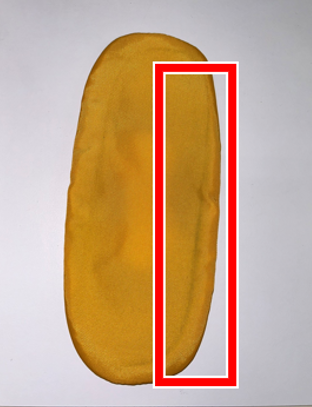
\includegraphics[keepaspectratio, width=0.8\linewidth, height=\linewidth]{figures/caring_brush_pad/10~15Akousatu.png}
        \caption{汚れに偏りなし}
        \label{fig:labelX}
    \end{subfigure}
    \begin{subfigure}[htbp]{0.3\linewidth}
        \centering
        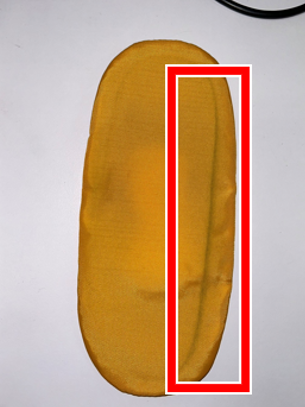
\includegraphics[keepaspectratio, width=0.8\linewidth, height=\linewidth]{figures/caring_brush_pad/10~15Bkousatu.png}
        \caption{汚れに偏りあり}
        \label{fig:labelY}
    \end{subfigure}
    \caption{10~15投使用}
    \label{fig:label}
\end{figure}

Fig.\ref{fig:labelX}とFig.\ref{fig:labelY}を比較したときにFig.\ref{fig:labelX}の方がブラシパッドの右側が汚い
ことが分かる.このことから,何投か使用した後にブラシパッドの倒す方向を逆にすることで,左右に偏りなく使用することが
できる.
\\

\section{色の違い}
デジタルマイクロスコープを用いて撮影した表面繊維の色をRGB値で数値化し,それを基にHSV値に変換した.HSV値を見ると
彩度(S)の値が使用回数が多くなるほど小さくなっていった.このことから使用回数が多いほど色が薄くなっている
ことが分かる.表面繊維の観察で考えたように,繊維がフィブリル化したことで色が薄くなったと考える.

\end{document}